\documentclass[a4paper, table]{article}



\newcommand\reportsubject  {Laboratoria Algorytmów i Struktur Danych}
\newcommand\reporttitle    {Drzewa przeszukiwań binarnych \\BST i drzewa samobalansujące}
\newcommand\reportsubtitle {Projekt 2 - opis i wymagania}
\newcommand\grouptutor     {Dominik Piotr Witczak}
\newcommand\projectdate    {26.kwi}
\newcommand\raportdate     {03.maj}




% Useful packages, sorted so packages of similar functionality are grouped together. Not all are essential to make the document work, however an effort was made to make this list as minimalistic as possible. Feel free to add your own!

% Essential for making this template work are graphicx, float, tabularx, tabu, tocbibind, titlesec, fancyhdr, xcolor and tikz. 

% Not essential, but you will have to debug the document a little bit when removing them are amsmath, amsthm, amssymb, amsfonts, caption, subcaption, appendix, enumitem, hyperref and cleveref.

% inputenc, lipsum, booktabs, geometry and microtype are not required, but nice to have.

\usepackage[T1]{fontenc}
\usepackage[polish]{babel}
\usepackage[utf8]{inputenc}
\usepackage{amsmath, amsthm, amssymb, amsfonts} % Nicer mathematical typesetting
\usepackage{multicol}
\usepackage{lipsum} % Creates dummy text lorem ipsum to showcase typsetting 
\usepackage{algorithm}
\usepackage{algpseudocode}
\usepackage{amsmath}
\usepackage{graphicx} % Allows the use of \begin{figure} and \includegraphics
\usepackage{float} % Useful for specifying the location of a figure ([H] for ex.)
\usepackage{caption} % Adds additional customization for (figure) captions
\usepackage{subcaption} % Needed to create sub-figures

\usepackage[nottoc,numbib]{tocbibind} % Automatically adds bibliography to ToC
\usepackage{titlesec} % Used to create custom section and subsection titles
\usepackage{titletoc} % Used to create a custom ToC
\usepackage{appendix} % Any chapter after \appendix is given a letter as index
\usepackage{fancyhdr} % Adds customization for headers and footers
\usepackage{hyperref} % Allows links and makes references and the ToC clickable
\usepackage[noabbrev, capitalise]{cleveref} % Easier referencing using \cref{<label>} instead of \ref{}
%\usepackage{fancyhdr}
%\pagestyle{fancy}

\usepackage{xcolor} % Predefines additional colors and allows user defined colors
\usepackage{tikz} % Useful for drawing images, used for creating the frontpage
\usetikzlibrary{positioning} % Additional library for relative positioning 
\usetikzlibrary{calc} % Additional library for calculating within tikz
\usetikzlibrary{shapes.geometric}
\usetikzlibrary{decorations.text}

% Defines a command used by tikz to calculate some coordinates for the front-page
\makeatletter
\newcommand{\gettikzxy}[3]{%
  \tikz@scan@one@point\pgfutil@firstofone#1\relax
  \edef#2{\the\pgf@x}%
  \edef#3{\the\pgf@y}%
}
\makeatother

% For terminal
\usepackage{fancyvrb,minted,tcolorbox}
\tcbuselibrary{skins,breakable,breakable}
\tcbuselibrary{minted}

% From previous

%Tworzenie wykresów bezpośrednio w LaTeXu
\usepackage{pgfplots}
%Pozwala dodać opcję H dlo figur, dzięki czemu mamy absolutną kontrolę gdzie się mają pojawić
\usepackage{float}
%Ustawianie marginesu 1 cal lub 0.5 cala to najlepsza opcja. Standardowe 1.5 cala nadaje się dla książek ale dla sprawozdań już mniej
\usepackage[margin=1in]{geometry}
\pgfplotsset{
	width=8cm, height=7cm, ymin=0, xmin=2047, xmax=32768, grid=both, %wymiary osi
	xticklabel style={rotate=45, anchor=near xticklabel},  %liczby na osi X pod kątem 45*
	x label style={at={(axis description cs:0.5,-0.03)}}, %legenda osi X wyśrodkowana, lekko obniżona
	y label style={at={(axis description cs:-0.1,0.4)}}
}
%\fancyhead[L]{
\includegraphics[width=10cm]{Figures/PP-PUT-WORD.png}} % Loads in the preamble 
\newcommand\reporttitle{Konspekt}
\newcommand\reportsubtitle{course code, name - Qx (202x)}
\definecolor{PUT-Blue}{HTML}{00618E}
\definecolor{Light-Gray}{HTML}{F5F3F1}
\definecolor{Gray}{HTML}{A5A29D}
\definecolor{Medium-Gray}{HTML}{52514F}
\definecolor{Dark-Gray}{HTML}{21201F}

% Change bullet style for level 1, 2 and 3 respectively for enumerate
\renewcommand{\labelenumi}{\textbf{\textcolor{PUT-Blue}{\arabic*.}}}% level 1
\renewcommand{\labelenumii}{\textbf{\textcolor{PUT-Blue}{[\alph*]}}}% level 2
\renewcommand{\labelenumiii}{\textbf{\textcolor{PUT-Blue}{\roman*.}}}% level 3

\renewcommand{\labelitemi}{\textbf{\textcolor{PUT-Blue}{$\circ$}}}% level 1


\newcommand{\putbf}[1]{\textbf{\textcolor{PUT-Blue}{#1}}}

% Formats section, subsection and subsubsection titles respectively 
\titleformat{\section}{\sffamily\color{PUT-Blue}\Large\bfseries}{\thesection\enskip\color{gray}\textbar\enskip}{0cm}{} % Formats section titles

\titleformat{\subsection}{\sffamily\color{PUT-Blue}\large\bfseries}{\thesubsection\enskip\color{gray}\textbar\enskip}{0cm}{} % Formats subsection titles

\titleformat{\subsubsection}{\sffamily\color{PUT-Blue}\bfseries}{\thesubsubsection\enskip\color{gray}\textbar\enskip}{0cm}{} % Formats subsubsection titles

% Removes indent when starting a new paragraph
\setlength\parindent{0pt}

\definecolor{terminalColor}{RGB}{38,50,56}
\definecolor{Button1}{RGB}{254,94,86}
\definecolor{Button2}{RGB}{254,188,45}
\definecolor{Button3}{RGB}{38,202,59} % Loads in the preamble 



\begin{document}
\begin{titlepage}

  \begin{tikzpicture}[remember picture,overlay]
    % Default apex angle 30 degrees
    \node(left-triagle)[isosceles triangle,
        isosceles triangle apex angle=90,
        fill=Light-Gray,
        minimum size =0.6\textheight] (T.west) at (current page.north west){};

    \node(bottom-triagle)[isosceles triangle, name=bottomtriangle,
        isosceles triangle apex angle=90, rotate=90,
        fill=Light-Gray,
        minimum height=40.05cm] () at ([xshift=-9cm]current page.south east){};

    \node(bottom-rectangle)[rectangle,
        fill=Light-Gray, minimum height=47cm, minimum width=18cm] () at (current page.south east)
        {};

 \node[inner sep=0pt] (logo) at ([xshift=2.5cm, yshift=-2.5cm]current page.north west)
    {
\includegraphics[width= 0.25\textwidth]{Figures/PP-PUT-LOGO.png}};

\node[text width = 0.8\textwidth](subject) at (16,-4){\sffamily\Large \reportsubject};
\node[text width = 0.8\textwidth, yshift = 0.75cm, xshift= -1.15cm, below = of subject](subtitle){\textcolor{PUT-Blue}{\sffamily\Large \reportsubtitle}};
\node[text width = 0.8\textwidth, yshift = 0.75cm, xshift= -1.15cm, below = of subtitle](title) {\textcolor{PUT-Blue}{\sffamily\Huge\reporttitle}};
\node[text width = 0.8\textwidth, yshift = 0.75cm, xshift= -1.25cm, below = of title](tutor){\sffamily\Large Prowadzący: \putbf{\grouptutor} };
\node[text width = 0.8\textwidth, yshift = 0.75cm, xshift= -1.15cm, below = of tutor](date1){\sffamily\Large Termin oddania projektu: \putbf{\projectdate}    };
\node[text width = 0.8\textwidth, yshift = 0.75cm, xshift= -1.15cm, below = of date1](date2){\sffamily\Large Termin oddania sprawozdania: \putbf{\raportdate} };



 \node[inner sep=0pt, anchor=west] (logo2) at ([xshift=1.2cm, yshift=2.5cm]current page.south west)
    {
\includegraphics[width= 0.6\textwidth]{Figures/PP-PUT-WORD}};

  \end{tikzpicture}

\end{titlepage} % Loads in the preamble 
\newpage
  \begin{tikzpicture}[remember picture,overlay]
    % Default apex angle 30 degrees
    \node(bottom-rectangle)[rectangle,
        fill=Light-Gray, minimum height=5cm, minimum width=2\textwidth] () at (current page.north)
        {};
    
    \node(left-triagle)[isosceles triangle,
        isosceles triangle apex angle=90,
        fill=Light-Gray,
        minimum size =0.4\textheight] (T.west) at (current page.north west){};

    \node(bottom-rectangle)[rectangle,
        fill=Light-Gray, minimum height=5cm, minimum width=2\textwidth] () at (current page.south)
        {};

    \node(left-triagle)[isosceles triangle,
        isosceles triangle apex angle=90, rotate=90,
        fill=Light-Gray,
        minimum size =0.4\textheight] (T.west) at (current page.south east){};


    \node[inner sep=0pt, anchor=west] (logo) at ([xshift=1.2cm, yshift=-1.5cm]current page.north west)
    {
\includegraphics[width= 0.4\textwidth]{Figures/PP-PUT-WORD.png}};

    \node[inner sep=0pt, anchor=center] (logo2) at ([xshift=-1.6cm, yshift=1.7cm]current page.south east)
    {
\includegraphics[width= 2.2cm]{Figures/PP-PUT-WIIT-LOGO.png}};


    \draw [double distance=4mm,
           double=gray,
           draw opacity=0,
           rotate=150,
           anchor=center,
           postaction={
                decorate,
                decoration={
                      raise=-1ex,
                      text along path, 
                      reverse path,
                      text align={fit to path stretching spaces},
                      text={|\ttfamily\footnotesize\color{black}|Kierunek\space Informatyka\space |\ttfamily\footnotesize\color{gray}|Wydzial\space Informatyki\space i\space Telekomunikacji}
                }
           }
        ] (logo2.center) circle (1.4cm);
    
  \end{tikzpicture}
\section{Zadanie}
Zaimplementuj algorytm konstruowania \textbf{drzewa AVL} metodą \textbf{połowienia binarnego} oraz algorytm konstruowania \textbf{drzewa BST} z ciągu liczb. 


\begin{figure} [H]
    \noindent\resizebox{\textwidth}{!}{
\centering
\begin{subfigure}{0.4\textwidth}
    \centering
    \newtcblisting{TcblistingMintedTerminal}[0]{listing engine=minted,minted style=native,
    minted language=python,enhanced,
    minted options={fontsize=\tiny},  
    colback=terminalColor,colframe=terminalColor,listing only, title=\tikz {
        \node[circle,fill=Button1,inner sep=3pt] (c) at (0,0){};
        \node[circle,fill=Button2,inner sep=3pt] (c) at (0.5,0){};
        \node[circle,fill=Button3,inner sep=3pt] (c) at (1,0){};
    } ~~~~~~Terminal
}

\newenvironment{TikzTreeStyle}
{ % Create enviroment - a tikzpicture with my styling for nodes
    \begin{tikzpicture}
        [level distance=10mm,
        every node/.style={fill=red!60,circle,inner sep=1pt, minimum size=6mm},
        level 1/.style={sibling distance=20mm,nodes={fill=red!45}},
        level 2/.style={sibling distance=10mm,nodes={fill=red!30}},
        level 3/.style={sibling distance=5mm,nodes={fill=red!25}}]
}
{ % Close enviroment
    \end{tikzpicture}
}

\begin{TcblistingMintedTerminal}
>>>  ./program --tree AVL <<< 7 2 5 10 12 13 6 9
 nodes> 7
insert> 2 5 10 12 13 6 9
Sorted: 2, 5, 6, 9, 10, 12, 13
Median: 9
action>
\end{TcblistingMintedTerminal}

\begin{TikzTreeStyle}
  \node {9}
    child {node {5}
      child {node {2}}
      child {node {6}}
    }
    child {node {12}
      child {node {10}}
      child {node {13}}
    };
    \path[draw=none] (0,-2) -- (0,14mm); %Set tikzpicture height to 34mm
\end{TikzTreeStyle} 
    \caption{Tworzenie drzewa AVL}
    \label{fig:avl:create}
\end{subfigure}
\hfill
\begin{subfigure}{0.4\textwidth}
    \centering
    \newtcblisting{TcblistingMintedTerminal}[0]{listing engine=minted,minted style=native,
    minted language=python,enhanced,
    minted options={fontsize=\tiny},  
    colback=terminalColor,colframe=terminalColor,listing only, title=\tikz {
        \node[circle,fill=Button1,inner sep=3pt] (c) at (0,0){};
        \node[circle,fill=Button2,inner sep=3pt] (c) at (0.5,0){};
        \node[circle,fill=Button3,inner sep=3pt] (c) at (1,0){};
    } ~~~~~~Terminal
}

\newenvironment{TikzTreeStyle}
{ % Create enviroment - a tikzpicture with my styling for nodes
    \begin{tikzpicture}
        [level distance=10mm,
        every node/.style={fill=red!60,circle,inner sep=1pt, minimum size=6mm},
        level 1/.style={sibling distance=20mm,nodes={fill=red!45}},
        level 2/.style={sibling distance=10mm,nodes={fill=red!30}},
        level 3/.style={sibling distance=5mm,nodes={fill=red!25}}]
}
{ % Close enviroment
    \end{tikzpicture}
}

\begin{TcblistingMintedTerminal}
>>>  ./program --tree BST <<< 7 2 5 10 12 13 6 9
 nodes> 7
insert> 2 5 10 12 13 6 9
Inserting: 2, 5, 10, 12, 13, 6, 9
action>

\end{TcblistingMintedTerminal}

\begin{TikzTreeStyle}
\node {2}
child[missing]
child 
{ node {5}
  child
  { node {6}
    child[missing]
    child { node {9} } }
  child 
  { node {12}
    child { node {10} }
    child { node {13} } }
};
\path[draw=none] (0,-3) -- (0,4mm); %Set tikzpicture height to 34mm
\end{TikzTreeStyle} 
    \caption{Tworzenie drzewa BST}
    \label{fig:bst:create}
\end{subfigure}
}
\end{figure}

\section{Menu}
Kiedy oczekujesz od użytkownika wprowadzenia danych, wyświetl odpowiedni znak zachęty (np. `nodes>`) .

% ' nodes>' - do wprowadzenia ilości węzłów które użytkownik ma zamiar wpisać,

% `insert>` - do wporwadzenia węzłów do dodania,

% `remove>` - do wprowadzenia węzłów do usunięcia,

% `action>` - do wprowadzenia kolejnej akcji. 

Akcje wpisywane będą w postaci ciągów znaków (Print, Remove, Delte, Export, Rebalance, Exit)

\begin{tcblisting}{listing engine=minted,minted style=native,
    minted language=python,enhanced,
    minted options={fontsize=\tiny},  
    colback=terminalColor,colframe=terminalColor,listing only, title=\tikz {
        \node[circle,fill=Button1,inner sep=3pt] (c) at (0,0){};
        \node[circle,fill=Button2,inner sep=3pt] (c) at (0.5,0){};
        \node[circle,fill=Button3,inner sep=3pt] (c) at (1,0){};
    } ~~~~~~Terminal}
>>>  ./program --tree AVL <<< 2, 5, 10, 12, 13, 6, 9
 nodes> 7
insert> 2 5 10 12 13 6 9
action> Help
Help        Show this message
Print       Print the tree usin In-order, Pre-order, Post-order
Remove      Remove elements of the tree 
Delete      Delete whole tree
Export      Export the tree to tickzpicture
Rebalance   Rebalance the tree
Exit        Exits the program (same as ctrl+D)
action> Print
...prints the tree...
action> Remove
remove> 10 12
action> Rebalance
(ctrl + D)
Program exited with status: 0
>>>
\end{tcblisting}

Program powinien także obsługiwać podawanie tzw. heredoc oraz `przekierowanie z pliku`. Ale nie martwcie się, jeśli program da się wpisać z palca, to obsłuży on także `heredoc` oraz `przekierowanie z pliku`.


\begin{figure}[H]
\begin{subfigure}{0.48\textwidth}
    \centering
\begin{tcblisting}{listing engine=minted,minted style=native,
    minted language=python,enhanced,
    minted options={fontsize=\tiny},  
    colback=terminalColor,colframe=terminalColor,listing only, title=\tikz {
        \node[circle,fill=Button1,inner sep=3pt] (c) at (0,0){};
        \node[circle,fill=Button2,inner sep=3pt] (c) at (0.5,0){};
        \node[circle,fill=Button3,inner sep=3pt] (c) at (1,0){};
    } ~~~~~~Terminal}
>>>  ./program --tree AVL << EOD
> 7
> 2 5 10 12 13 6 9
> Print
> Exit
> EOD
\end{tcblisting}
    \caption{Heredoc}
    \label{fig:avl:create}
\end{subfigure}
\hfill
\begin{subfigure}{0.48\textwidth}
    \centering
\begin{tcblisting}{listing engine=minted,minted style=native,
    minted language=python,enhanced,
    minted options={fontsize=\tiny},  
    colback=terminalColor,colframe=terminalColor,listing only, title=\tikz {
        \node[circle,fill=Button1,inner sep=3pt] (c) at (0,0){};
        \node[circle,fill=Button2,inner sep=3pt] (c) at (0.5,0){};
        \node[circle,fill=Button3,inner sep=3pt] (c) at (1,0){};
    } ~~~~~~Terminal}
>>> more plik.txt
7
2 5 10 12 13 6 9
Print
Exit
>>>  ./program --tree AVL < plik.txt
\end{tcblisting}
    \caption{Przekierowanie z pliku}
    \label{fig:bst:create}
\end{subfigure}
\end{figure}
 % Loads in the preamble 
\newpage
  \begin{tikzpicture}[remember picture,overlay]
    % Default apex angle 30 degrees
    \node(bottom-rectangle)[rectangle,
        fill=Light-Gray, minimum height=5cm, minimum width=2\textwidth] () at (current page.north)
        {};
    
    \node(left-triagle)[isosceles triangle,
        isosceles triangle apex angle=90,
        fill=Light-Gray,
        minimum size =0.4\textheight] (T.west) at (current page.north west){};

    \node(bottom-rectangle)[rectangle,
        fill=Light-Gray, minimum height=5cm, minimum width=2\textwidth] () at (current page.south)
        {};

    \node(left-triagle)[isosceles triangle,
        isosceles triangle apex angle=90, rotate=90,
        fill=Light-Gray,
        minimum size =0.4\textheight] (T.west) at (current page.south east){};


    \node[inner sep=0pt, anchor=west] (logo) at ([xshift=1.2cm, yshift=-1.5cm]current page.north west)
    {
\includegraphics[width= 0.4\textwidth]{Figures/PP-PUT-WORD.png}};

    \node[inner sep=0pt, anchor=center] (logo2) at ([xshift=-1.6cm, yshift=1.7cm]current page.south east)
    {
\includegraphics[width= 2.2cm]{Figures/PP-PUT-WIIT-LOGO.png}};


    \draw [double distance=4mm,
           double=gray,
           draw opacity=0,
           rotate=150,
           anchor=center,
           postaction={
                decorate,
                decoration={
                      raise=-1ex,
                      text along path, 
                      reverse path,
                      text align={fit to path stretching spaces},
                      text={|\ttfamily\footnotesize\color{black}|Kierunek\space Informatyka\space |\ttfamily\footnotesize\color{gray}|Wydzial\space Informatyki\space i\space Telekomunikacji}
                }
           }
        ] (logo2.center) circle (1.4cm);
    
  \end{tikzpicture}
\newtcblisting{TcblistingMintedPython}[0]{listing engine=minted,minted style=native,
    minted language=python,enhanced,
    minted options={fontsize=\tiny},  
    colback=terminalColor,
    colframe=terminalColor,
    listing only,
    title= \tikz {
        \node[circle,inner sep=0pt] at (0,0){
\includegraphics[width=0.2cm]{Figures/PYTHON-LOGO.png}};;
    } ~~~~~~Python
}
\section{Operacje na drzewach}

\begin{multicols}{2}
  \begin{enumerate}[series=actions]
    \item \textcolor{PUT-Blue}{\putbf{Wyszukiwanie}} w drzewie elementu o najmniejszej i największej wartości
    \begin{figure} [H]
        \centering
        \newtcblisting{TcblistingMintedTerminal}[0]{listing engine=minted,minted style=native,
    minted language=python,enhanced,
    minted options={fontsize=\tiny},  
    colback=terminalColor,colframe=terminalColor,listing only, title=\tikz {
        \node[circle,fill=Button1,inner sep=3pt] (c) at (0,0){};
        \node[circle,fill=Button2,inner sep=3pt] (c) at (0.5,0){};
        \node[circle,fill=Button3,inner sep=3pt] (c) at (1,0){};
    } ~~~~~~Terminal
}

\newenvironment{TikzTreeStyle}
{ % Create enviroment - a tikzpicture with my styling for nodes
    \begin{tikzpicture}
        [level distance=10mm,
        every node/.style={fill=red!60,circle,inner sep=1pt, minimum size=6mm},
        level 1/.style={sibling distance=20mm,nodes={fill=red!45}},
        level 2/.style={sibling distance=10mm,nodes={fill=red!30}},
        level 3/.style={sibling distance=5mm,nodes={fill=red!25}}]
}
{ % Close enviroment
    \end{tikzpicture}
}

\begin{TcblistingMintedTerminal}
>>>  ./program --tree AVL <<< 2, 5, 10, 12, 13, 6, 9
Sorted: 2, 5, 6, 9, 10, 12, 13
Median: 9
action> FindMinMax
Min: 2
Max: 13
\end{TcblistingMintedTerminal}

\begin{TikzTreeStyle}
  \node {9}
    child {node {5} edge from parent [draw=green]
      child {node {2} edge from parent [draw=green] }
      child {node {6} edge from parent [draw=black] }
    }
    child {node {12} edge from parent [draw=red]
      child {node {10} edge from parent [draw=black] }
      child {node {13} edge from parent [draw=  red] }
    };
\end{TikzTreeStyle} 
        \caption{Wyszukiwanie elementu o największej i najmniejszej wartości}
        \label{fig:tree:search}
    \end{figure}
    
    \item \textcolor{PUT-Blue}{\putbf{Wypisanie}} wszystkich elementów drzewa w porządku in-order, pre-order oraz post-order. [Dla chętnych] wypisanie drzewa do tickzpicture
    \begin{figure} [H]
        \centering
        \newtcblisting{TcblistingMintedTerminal}[0]{listing engine=minted,minted style=native,
    minted language=python,enhanced,
    minted options={fontsize=\tiny},  
    colback=terminalColor,colframe=terminalColor,listing only, title=\tikz {
        \node[circle,fill=Button1,inner sep=3pt] (c) at (0,0){};
        \node[circle,fill=Button2,inner sep=3pt] (c) at (0.5,0){};
        \node[circle,fill=Button3,inner sep=3pt] (c) at (1,0){};
    } ~~~~~~Terminal
}

\newenvironment{TikzTreeStyle}
{ % Create enviroment - a tikzpicture with my styling for nodes
    \begin{tikzpicture}
        [level distance=10mm,
        every node/.style={fill=red!60,circle,inner sep=1pt, minimum size=6mm},
        level 1/.style={sibling distance=20mm,nodes={fill=red!45}},
        level 2/.style={sibling distance=10mm,nodes={fill=red!30}},
        level 3/.style={sibling distance=5mm,nodes={fill=red!25}}]
}
{ % Close enviroment
    \end{tikzpicture}
}

\begin{TcblistingMintedTerminal}
action> Print
  In-order:  2,  5,  6,  9, 10, 12, 13
Post-order:  2,  6,  5, 10, 13, 12,  9
 Pre-order:  9,  5,  2,  6, 12, 10, 13
\end{TcblistingMintedTerminal}

\begin{TikzTreeStyle}
  \node {9}
    child {node {5}
      child {node {2} }
      child {node {6} }
    }
    child {node {12}
      child {node {10} }
      child {node {13} }
    };
\end{TikzTreeStyle}
        \caption{Wypisywanie zawartości drzewa (Print)}
        \label{fig:tree:search}
    \end{figure}

    \item \textcolor{PUT-Blue}{\putbf{Narysowanie}} drzewa w tickzpicture \putbf{(dodatkowy punkt)}
    \begin{figure} [H]
        \centering
        \begin{TcblistingMintedPython}
def export():
    if not node.left and not node.right:
        return f"node {node.value}" 
    l_str = f"child {export(node.l)}" if node.l else "child[missing]"
    r_str = f"child {export(node.r)}" if node.r else "child[missing]"
    return f" node {node.value} \{{l_str}\} \{{r_str}\}\"

def main():
    return f"\\{export(tree_root)}"
\end{TcblistingMintedPython}
        \caption{Przykładowa implementacja}
        \label{fig:tree:export:code}
    \end{figure}

    \item \textcolor{PUT-Blue}{\putbf{Usuwanie}} z drzewa ciągu elementów podanych przez użytkownika. Dopuszczalne jest:
    \begin{enumerate}[label=(\alph*)]
        \item usuwanie liści,
        \item usuwanie elementu z jednym potomkiem, 
        \item usuwanie elemntu z dwoma potomkami.
    \end{enumerate}   
    \begin{figure} [H]
        \centering
        \newtcblisting{TcblistingMintedTerminal}[0]{listing engine=minted,minted style=native,
    minted language=python,enhanced,
    minted options={fontsize=\tiny},  
    colback=terminalColor,colframe=terminalColor,listing only, title=\tikz {
        \node[circle,fill=Button1,inner sep=3pt] (c) at (0,0){};
        \node[circle,fill=Button2,inner sep=3pt] (c) at (0.5,0){};
        \node[circle,fill=Button3,inner sep=3pt] (c) at (1,0){};
    } ~~~~~~Terminal
}

\newenvironment{TikzTreeStyle}
{ % Create enviroment - a tikzpicture with my styling for nodes
    \begin{tikzpicture}
        [level distance=10mm,
        every node/.style={fill=red!60,circle,inner sep=1pt, minimum size=6mm},
        level 1/.style={sibling distance=20mm,nodes={fill=red!45}},
        level 2/.style={sibling distance=10mm,nodes={fill=red!30}},
        level 3/.style={sibling distance=5mm,nodes={fill=red!25}}]
}
{ % Close enviroment
    \end{tikzpicture}
}

\begin{TcblistingMintedTerminal}
action> Delete
 nodes> 3
delete> 2 5 10

\end{TcblistingMintedTerminal}

\begin{TikzTreeStyle}
\node[draw=black,dash pattern= on 3pt off 5pt,thick,postaction={draw,red,dash pattern= on 3pt off 5pt,dash phase=4pt,thick}] at (0,0) {9} 
child {node {5}
  child {node {2}}
  child {node [draw=black,dash pattern= on 3pt off 5pt,thick,postaction={draw,green,dash pattern= on 3pt off 5pt,dash phase=4pt,thick}] {6}}
}
child {node {12}
  child {node {10}}
  child {node {13}}
};

\node at (4,0) (c) {6} 
child {node {5}
  child {node {2} }
  child [missing]
}
child {node [draw=black,dash pattern= on 3pt off 5pt,thick,postaction={draw,red,dash pattern= on 3pt off 5pt,dash phase=4pt,thick}] {12}
  child {node [draw=black,dash pattern= on 3pt off 5pt,thick,postaction={draw,green,dash pattern= on 3pt off 5pt,dash phase=4pt,thick}] {10}}
  child {node {13}}
};

\node at (0,-3.5) (b) {6} 
child {node {5}
  child {node {2} }
  child [missing]
}
child {node {10}
  child[missing]
  child {node [draw=black,dash pattern= on 3pt off 5pt,thick,postaction={draw,red,dash pattern= on 3pt off 5pt,dash phase=4pt,thick}] {13}}
};


\node at (4,-3.5) (a) {6} 
child {node {5}
  child {node {2} }
  child [missing]
}
child {node {10}};

%Add arrows
\path[double, draw=black, ->] (1.5,  -1) -- (2.5,  -1);
\path[double, draw=black, ->] (2.4,-2.7) -- (1.6,  -3.2);
\path[double, draw=black, ->] (1.5,-4.5) -- (2.5,-4.5);

\node[draw=none,fill=none] (1) [label=above:{(c)}] at (2,   -1) {};
\node[draw=none,fill=none] (1) [label=above:{(b)}] at (2, -3.2) {};
\node[draw=none,fill=none] (1) [label=above:{(a)}] at (2, -4.5) {};
    
\end{TikzTreeStyle} 
        \caption{Usuwanie elementów}
        \label{fig:tree:search}
    \end{figure}

    \item \textcolor{PUT-Blue}{\putbf{Usunięcie}} całego drzewa element po elemencie metodą post-order 
    \begin{figure} [H]
        \centering
        \newtcblisting{TcblistingMintedTerminal}[0]{listing engine=minted,minted style=native,
    minted language=python,enhanced,
    minted options={fontsize=\tiny},  
    colback=terminalColor,colframe=terminalColor,listing only, title=\tikz {
        \node[circle,fill=Button1,inner sep=3pt] (c) at (0,0){};
        \node[circle,fill=Button2,inner sep=3pt] (c) at (0.5,0){};
        \node[circle,fill=Button3,inner sep=3pt] (c) at (1,0){};
    } ~~~~~~Terminal
}

\newenvironment{TikzTreeStyle}
{ % Create enviroment - a tikzpicture with my styling for nodes
    \begin{tikzpicture}
        [level distance=10mm,
        every node/.style={fill=red!60,circle,inner sep=1pt, minimum size=6mm},
        level 1/.style={sibling distance=20mm,nodes={fill=red!45}},
        level 2/.style={sibling distance=10mm,nodes={fill=red!30}},
        level 3/.style={sibling distance=5mm,nodes={fill=red!25}}]
}
{ % Close enviroment
    \end{tikzpicture}
}

\begin{TcblistingMintedTerminal}
action> Delete All
Deleting: 2 5 10 6
Tree succesfully removed
\end{TcblistingMintedTerminal}


\begin{TikzTreeStyle}
%  _   _                             _            __  _     _____                 
% | | | | _ __   _ __    ___  _ __  | |     ___  / _|| |_  |_   _|_ __  ___   ___ 
% | | | || '_ \ | '_ \  / _ \| '__| | |    / _ \| |_ | __|   | | | '__|/ _ \ / _ \
% | |_| || |_) || |_) ||  __/| |    | |___|  __/|  _|| |_    | | | |  |  __/|  __/
%  \___/ | .__/ | .__/  \___||_|    |_____|\___||_|   \__|   |_| |_|   \___| \___|
%        |_|    |_|                                                               
\node at (0,0)  {6} 
child {node {5}
  child {node [draw=black,dash pattern= on 3pt off 5pt,thick,postaction={draw,red,dash pattern= on 3pt off 5pt,dash phase=4pt,thick}] {2} }
  child [missing]
}
child {node {10}};

%  _   _                             ____   _         _      _     _____                 
% | | | | _ __   _ __    ___  _ __  |  _ \ (_)  __ _ | |__  | |_  |_   _|_ __  ___   ___ 
% | | | || '_ \ | '_ \  / _ \| '__| | |_) || | / _` || '_ \ | __|   | | | '__|/ _ \ / _ \
% | |_| || |_) || |_) ||  __/| |    |  _ < | || (_| || | | || |_    | | | |  |  __/|  __/
%  \___/ | .__/ | .__/  \___||_|    |_| \_\|_| \__, ||_| |_| \__|   |_| |_|   \___| \___|
%        |_|    |_|                            |___/                                     
\node at (4,0) (c) {6} 
child {node [draw=black,dash pattern= on 3pt off 5pt,thick,postaction={draw,red,dash pattern= on 3pt off 5pt,dash phase=4pt,thick}] {5}}
child {node {10}};

%  _                                 _            __  _     _____                 
% | |     ___ __      __ ___  _ __  | |     ___  / _|| |_  |_   _|_ __  ___   ___ 
% | |    / _ \\ \ /\ / // _ \| '__| | |    / _ \| |_ | __|   | | | '__|/ _ \ / _ \
% | |___| (_) |\ V  V /|  __/| |    | |___|  __/|  _|| |_    | | | |  |  __/|  __/
% |_____|\___/  \_/\_/  \___||_|    |_____|\___||_|   \__|   |_| |_|   \___| \___|
%
\node at (0,-3.5) (b) {6} 
child[missing]
child {node [draw=black,dash pattern= on 3pt off 5pt,thick,postaction={draw,red,dash pattern= on 3pt off 5pt,dash phase=4pt,thick}] {10}};

%  _                                 ____   _         _      _     _____                 
% | |     ___ __      __ ___  _ __  |  _ \ (_)  __ _ | |__  | |_  |_   _|_ __  ___   ___ 
% | |    / _ \\ \ /\ / // _ \| '__| | |_) || | / _` || '_ \ | __|   | | | '__|/ _ \ / _ \
% | |___| (_) |\ V  V /|  __/| |    |  _ < | || (_| || | | || |_    | | | |  |  __/|  __/
% |_____|\___/  \_/\_/  \___||_|    |_| \_\|_| \__, ||_| |_| \__|   |_| |_|   \___| \___|
%                                              |___/                                     
\node at (4,-3.5) (a) [draw=black,dash pattern= on 3pt off 5pt,thick,postaction={draw,red,dash pattern= on 3pt off 5pt,dash phase=4pt,thick}] {6};

%%%%%%%%%%%%%%%%%%%%%%%%%%%%%%%%%%%%%%%%%%%%%%%%%%%%%%%%%%%%%%%%%%%%%%%%
%   Add arrows 
%%%%%%%%%%%%%%%%%%%%%%%%%%%%%%%%%%%%%%%%%%%%%%%%%%%%%%%%%%%%%%%%%%%%%%%%
\path[double, draw=black, ->] (1.5,  -1) -- (2.5,  -1);
\path[double, draw=black, ->] (2.4,-2.7) -- (1.6,  -3.2);
\path[double, draw=black, ->] (1.5,-4.5) -- (2.5,-4.5);
    
\end{TikzTreeStyle} 
        \caption{Usuwanie drzewa}
        \label{fig:tree:search}
    \end{figure}

    
  \end{enumerate}
\end{multicols}



\newpage
  \begin{tikzpicture}[remember picture,overlay]
    % Default apex angle 30 degrees
    \node(bottom-rectangle)[rectangle,
        fill=Light-Gray, minimum height=5cm, minimum width=2\textwidth] () at (current page.north)
        {};
    
    \node(left-triagle)[isosceles triangle,
        isosceles triangle apex angle=90,
        fill=Light-Gray,
        minimum size =0.4\textheight] (T.west) at (current page.north west){};

    \node(bottom-rectangle)[rectangle,
        fill=Light-Gray, minimum height=5cm, minimum width=2\textwidth] () at (current page.south)
        {};

    \node(left-triagle)[isosceles triangle,
        isosceles triangle apex angle=90, rotate=90,
        fill=Light-Gray,
        minimum size =0.4\textheight] (T.west) at (current page.south east){};


    \node[inner sep=0pt, anchor=west] (logo) at ([xshift=1.2cm, yshift=-1.5cm]current page.north west)
    {
\includegraphics[width= 0.4\textwidth]{Figures/PP-PUT-WORD.png}};

    \node[inner sep=0pt, anchor=center] (logo2) at ([xshift=-1.6cm, yshift=1.7cm]current page.south east)
    {
\includegraphics[width= 2.2cm]{Figures/PP-PUT-WIIT-LOGO.png}};


    \draw [double distance=4mm,
           double=gray,
           draw opacity=0,
           rotate=150,
           anchor=center,
           postaction={
                decorate,
                decoration={
                      raise=-1ex,
                      text along path, 
                      reverse path,
                      text align={fit to path stretching spaces},
                      text={|\ttfamily\footnotesize\color{black}|Kierunek\space Informatyka\space |\ttfamily\footnotesize\color{gray}|Wydzial\space Informatyki\space i\space Telekomunikacji}
                }
           }
        ] (logo2.center) circle (1.4cm);
    
  \end{tikzpicture}

\begin{enumerate}[resume=actions]
    \item \textcolor{PUT-Blue}{\putbf{Równoważenie}} drzewa element po elemencie metodą DSW

\newtcblisting{TcblistingMintedTerminal}[0]{listing engine=minted,minted style=native,
    minted language=python,enhanced,
    minted options={fontsize=\tiny},  
    colback=terminalColor,colframe=terminalColor,listing only, title=\tikz {
        \node[circle,fill=Button1,inner sep=3pt] (c) at (0,0){};
        \node[circle,fill=Button2,inner sep=3pt] (c) at (0.5,0){};
        \node[circle,fill=Button3,inner sep=3pt] (c) at (1,0){};
    } ~~~~~~Terminal
}

\begin{figure}[H]
    \begin{subfigure}{\textwidth}
\begin{TcblistingMintedTerminal}
>>>  ./program --tree AVL <<< 1, 2, 3, 6, 5, 4, 7
Inserting: 1, 2, 3, 6, 5, 4, 7
action> Rebalance
Pre-Order:  4, 2, 1, 3, 6, 5, 7,
\end{TcblistingMintedTerminal}
        \caption{Interfejs linii komend}
        \label{fig:tree:rebalance:code}
    \end{subfigure}

    \centering
    \begin{subfigure}{\textwidth}
        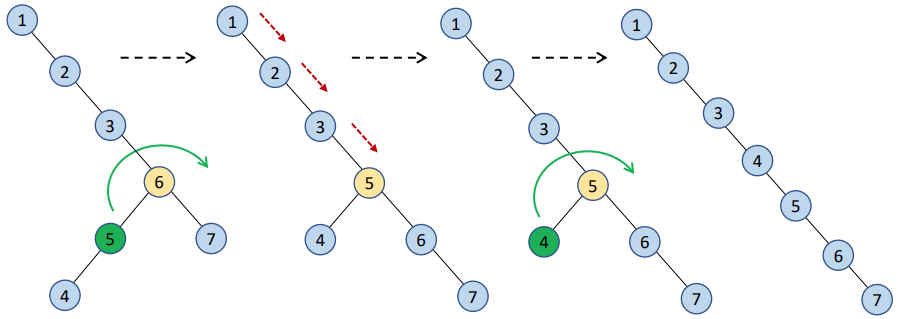
\includegraphics[width=\textwidth]{Figures/DSW-Phase1.png} 
        \caption{Faza pierwsza}
        \label{fig:tree:rebalance:phase1}
    \end{subfigure}

    \begin{subfigure}{\textwidth}
        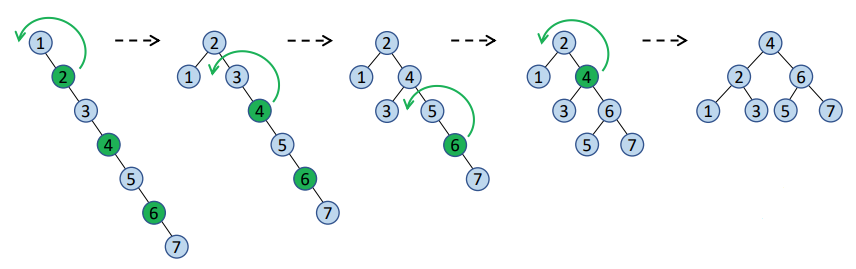
\includegraphics[width=\textwidth]{Figures/DSW-Phase2.png}
        \caption{Faza druga}
        \label{fig:tree:rebalance:phase2}
    \end{subfigure}
    \caption{Równoważenie metodą Day-Stout-Warren}
\end{figure}
    
\end{enumerate}

\section{Wymagania do oceny}
\begin{table}[H]
    \centering
    \begin{tabular}{|c|c|c|c|c|c|c|c|} \hline
    \multicolumn{2}{|c|}{Zadanie 1 - Tworzenie}& Zadanie 2 - Menu         & \multicolumn{5}{c|}{ Zadanie 3 - Operacje              }\\ \hline    
                                     BST & AVL & Zgodność ze specyfikacją & FindMinMax & Print & Remove     & RemoveAll & Rebalance \\ \hline
                                       1 & 3   & 2                        & 1          & 1     & \putbf{4} & 1         & \putbf{7}\\ \hline
    \end{tabular}
    \caption{Szczegółowa Punktacja}
    \label{tab:my_label}
\end{table}
\putbf{W sumie 20 punktów}. Dodatkowe punkty, poza skalą: 1 pkt za export drzewa do tickzpicture. Do 3 punktów za staranność wykonania projketu (np. czystość kodu, ekspertyza w języku czy używanie gita). 

\begin{table}[H]
    \centering
    \begin{tabular}{|c|c|c|c|c|c|c|c|} \hline
         2 & 3     & 3.5   & 4     & 4.5   & 5  & 5.5 \\ \hline
     do 11 & od 12 & od 14 & od 16 & od 18 & 20 & ponad 22\\ \hline
    \end{tabular}
    \caption{Szczegółowa Punktacja}
    \label{tab:my_label}
\end{table}

\newpage
\hspace{1em} % Skip for aesthetics
\section{Benchmark implementacji}
Ponownie przygotuję dla was generator danych wejściowych, które zapiszę do pliku.
Przygotuję też pliki zawierające polecenia które można przekazać do programu.

Tym razem \putbf{to po waszej stronie} leży \putbf{wykonanie pomiar czasu} - dlatego że musimy zmierzyć poszczególne metody, a nie czas trwania wykonywania całego programu. Z racji że mierzymy czas zegarowy, proszę o zrobienie po 4 pomiary i uśrednienie wyniku. Do pomiaru jest:

\begin{enumerate} [label=\putbf{(\alph*)}]
\item tworzenie drzewa AVL metodą połowienia binarnego, 
\item tworzenie drzewa BST poprzez wstawianie kolejno elementów (drzewo zdegnerowane),
\item wyszukiwanie elementów o minimalnej i maksymalnej wartości,
\item wypisywanie wszystkich elementów drzewa (in-order),
\item równoważenia drzewa BST.
\end{enumerate}

Postaram się jeszcze wymyślić sposób aby ułatwić wam mierzenie czasu, ale nie mogę nic obiecać. W razie czego poinformuję was na Discordzie.


  \begin{tikzpicture}[remember picture,overlay]
    % Default apex angle 30 degrees
    \node(bottom-rectangle)[rectangle,
        fill=Light-Gray, minimum height=5cm, minimum width=2\textwidth] () at (current page.north)
        {};
    
    \node(left-triagle)[isosceles triangle,
        isosceles triangle apex angle=90,
        fill=Light-Gray,
        minimum size =0.4\textheight] (T.west) at (current page.north west){};

    \node(bottom-rectangle)[rectangle,
        fill=Light-Gray, minimum height=5cm, minimum width=2\textwidth] () at (current page.south)
        {};

    \node(left-triagle)[isosceles triangle,
        isosceles triangle apex angle=90, rotate=90,
        fill=Light-Gray,
        minimum size =0.4\textheight] (T.west) at (current page.south east){};


    \node[inner sep=0pt, anchor=west] (logo) at ([xshift=1.2cm, yshift=-1.5cm]current page.north west)
    {
\includegraphics[width= 0.4\textwidth]{Figures/PP-PUT-WORD.png}};

    \node[inner sep=0pt, anchor=center] (logo2) at ([xshift=-1.6cm, yshift=1.7cm]current page.south east)
    {
\includegraphics[width= 2.2cm]{Figures/PP-PUT-WIIT-LOGO.png}};


    \draw [double distance=4mm,
           double=gray,
           draw opacity=0,
           rotate=150,
           anchor=center,
           postaction={
                decorate,
                decoration={
                      raise=-1ex,
                      text along path, 
                      reverse path,
                      text align={fit to path stretching spaces},
                      text={|\ttfamily\footnotesize\color{black}|Kierunek\space Informatyka\space |\ttfamily\footnotesize\color{gray}|Wydzial\space Informatyki\space i\space Telekomunikacji}
                }
           }
        ] (logo2.center) circle (1.4cm);
    
  \end{tikzpicture}
\section{Wymagania do sprawozdania}


\begin{itemize}[label={}]
\item \textcolor{PUT-Blue}{[1 pkt]} Zaprezentuj swój program (screenem utworzenia drzewa BST, AVL). Pokaż wizualizację utworzonych wykresów. Drzewo BST ma być niezbalansowane.  

\item \textcolor{PUT-Blue}{[1 pkt]} Na wizualizacjach oznacz liście, korzeń i węzły wewnętrzne.

\item \textcolor{PUT-Blue}{[4 pkt]} Wykonaj 3 wykresy (jeden wykres dla każdej z operacji: tworzenie struktury, wyszukanie min/max, wypisanie in-order) t=f(n) zależności czasu obliczeń t od liczby n elementów w drzewie. Na każdym wykresie przedstaw 2 krzywe - po jednej krzywej dla BST i AVL. 

\item \textcolor{PUT-Blue}{[4 pkt]} Wykonaj wykres t=f(n) zależności czasu równoważenia (t) od liczby elementów (n) w drzewie BST.

\item \textcolor{PUT-Blue}{Dodatkowy: [1 pkt]} Wykonaj sprawozdanie w LaTeXu :)

\item \textcolor{PUT-Blue}{Dodatkowy: [1 pkt]} Przedstaw wykresy w takim ułożeniu:

\begin{figure}[H]
    \centering
    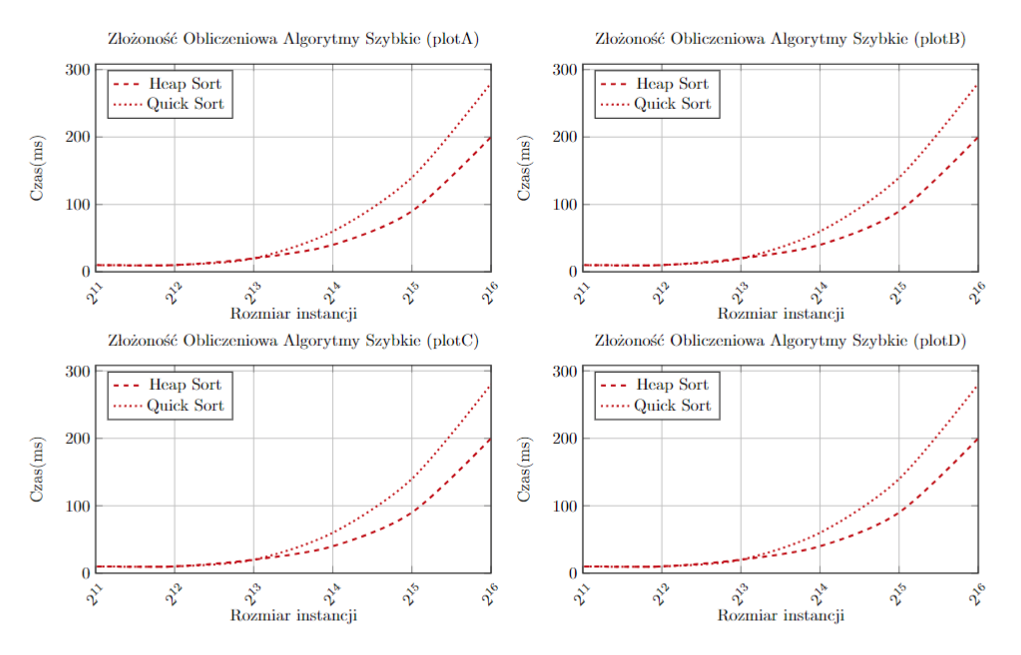
\includegraphics[width=0.4\textwidth]{Figures/Plots.png} 
    \caption{Ilustracja podzielona na 4 podwykresy}
    \label{fig:tree:rebalance:phase1}
\end{figure}

\putbf{W sumie 10 punktów}.
\begin{table}[H]
    \centering
    \begin{tabular}{|c|c|c|c|c|c|c|c|} \hline
         2 & 3     & 3.5   & 4     & 4.5   & 5   & 5.5      \\ \hline
      do 5 & 6     &     7  &    8  & 9     & 10 & 12 \\ \hline
    \end{tabular}
    \caption{Szczegółowa Punktacja}
    \label{tab:my_label}
\end{table}


\end{itemize}

 % Loads in the preamble 
\end{document}

% \documentclass[a4paper,12pt]{article}
% \usepackage{tikz}
% \usepackage[left=5.2cm,top=2cm,right=1.5cm,bottom=2cm,verbose,nohead,nofoot]{geometry}
% \usepackage{etoolbox}
% \usetikzlibrary{shapes.geometric}

% \begin{document}
%   \thispagestyle{empty}

% \end{document}